
  \documentclass{article}
\usepackage{graphicx} % Required for inserting images
\usepackage[margin=2cm]{geometry} 
\usepackage{multicol,amsmath, amssymb}
\usepackage{xcolor}
\usepackage{titlesec}

\titleformat{\subsection}
{\color{red}\normalfont\Large\bfseries}
{\thesubsection}{1em}{}

\titleformat{\subsubsection}
{\color{blue}\normalfont\large\bfseries}
{\thesubsubsection}{1em}{}

\titlespacing{\subsection}{0pt}{0pt}{0pt} % Adjust the spacing here
\titlespacing{\subsubsection}{0pt}{\baselineskip}{0pt} % Adjust the spacing here

\usepackage{fancyhdr}
\usepackage{hyperref} % For hyperlinks

% Define the URL for the footer
\newcommand{\myURL}{https://mohammedbilalns.github.io/Math-Demystified/}

% Set up fancy headers and footers
\pagestyle{fancy}
\fancyhf{} % Clear header and footer
\rfoot{\href{\myURL}{\myURL}} % Set the right part of the footer as a hyperlink

\begin{document}
\begin{center}
    {\LARGE \textbf{COMPLEX NUMBERS AND QUADRATIC EQUATIONS} }
\end{center}

\begin{multicols}{2}
  we have studied linear equations in one and two variables and quadratic equations in one variable. We have seen that the equation $x^2 + 1 = 0$ has no real solution since the root of a negative number does not exist in a real number. So, we need to extend the real number system to a larger number system to accommodate such numbers.

\subsection*{Complex Numbers}
  A number of the form $a + ib$, where a and b are real numbers and $i = \sqrt{-1}$.
Usually, a complex number is denoted by $z$, $a$ is the real part of $z$ denoted by $Re(z)$ and $b$ is the imaginary part of $z$ denoted by $Im(z)$.Two complex numbers $z_1 = a + ib$ and $z_2 = c + id$ are equal if $a = c$ and $b = d.$

For example, $2 + i3, (– 1) + i \sqrt{3} , 4 + i \frac{-1}{11} $ are complex numbers.

\subsubsection*{ Algebra of Complex Numbers}

\begin{enumerate}
    \item \textbf{Addition of two complex numbers:}
    
    Let $z_1 = a + ib$ and $z_2 = c + id$ be two complex numbers. Then the sum $z_1 + z_2$ is obtained by adding the real and imaginary parts.

    For example $(2 + i3) + (– 6 +i5) = (2 – 6) + i (3 + 5) = – 4 + i 8$. 

    The addition of complex numbers satisfy the following properties: \begin{enumerate}
        \item $z_1 + z+_2$ is a complex number (Closure)
        \item  $z_1 + z_2 = z_2 + z_1$ (commutative)
        \item  $z_1 + (z_2 + z_3) = (z_1 + z_2) + z_3$ (associative)
        \item $0 + i0$ is the identity element.
        \item  $-z$ is the inverse of $z$.
        
    \end{enumerate}
    \item \textbf{Difference of two complex numbers:} Given any two complex numbers $z_1$ and
$z_2$, the difference $z_1 – z_2$ is defined as follows:
$z_1 – z_2 = z_1 + (– z_2)$

\item \textbf{Multiplication of two complex numbers:} Let $z_1 = a + ib$ and $z_2 = c + id$ be two complex numbers.
Then the product $z_1z_2$ is defined as follows:
$z_1z_2 = (ac – bd) + i(ad + bc)$.

For example, $(3 + i5) (2 + i6) = (3 \times 2 – 5 \times 6) + i(3 \times 6 + 5 \times 2) = – 24 + i28$

The multiplication of complex numbers possesses the following properties
\begin{enumerate}
    \item Product of two complex numbers is a complex number(closure)
    \item  $z_1z_2 = z_2z_1$ (commutative).
    \item  $z_1(z_2z_3) = (z_1z_2)z_3$ (associative).
    \item  $1 + i0$ is the identity element.
    \item $\frac{1}{z}$ is the inverse of z.
    \item $z_1(z_2 + z_3) = z_1z_2 + z_1z_3$ (distributive law)
    
\end{enumerate}
    \item \textbf{Division of two complex numbers:} Given any two complex numbers $z_1$ and $z_2$,
where $z_2 \not = $0 , the quotient $\frac{z_1}{z_2}$ is defined by
$$\frac{z_1}{z_2}=z_1 \times \frac{1}{z_2}$$

\item \textbf{Power of i:}In General $i^{4k} = 1, i^{4k+1} = i, i^{4k+2} = -1, i^{4k+3} = -i, i^{-1}=-i$

\item \textbf{The square roots of a negative real number:}

We have 
$$(\sqrt{3}i)^2=\sqrt{3}^2 i^2=3 \times -1 =-3$$
$$(\sqrt{-3}i)^2=\sqrt{-3}^2 i^2=3 \times -1 =-3$$

Therefor the square roots or -3 are $\sqrt{3}i$ and $-\sqrt{3}i$. In general if  a is a positive real number then 
$\sqrt{-a}=i\sqrt{a}$ and $-i\sqrt{a}$.

Therefore $\sqrt{a} \times \sqrt{b} \not = ab$ if both a and b are negative real numbers.

\item \textbf{Identities:}
\begin{itemize}
    \item $(z_1+z_2)^2=z_1^2+2z_1z_2+z_2^2$
    \item $(z_1-z_2)^2=z_1^2-2z_1z_2+z_2^2$
    \item $(z_1+z_2)^3=z_1^3+3z_1^2z_2+3z_2^2z_1+z_2^3$
    \item $(z_1-z_2)^3=z_1^3-3z_1^2z_2+3z_2^2z_1-z_2^3$
\end{itemize}

\end{enumerate}

\subsection*{The Modulus and the Conjugate of a Complex Number:}

Consider a complex number $z = a + ib$ . Then, the conjugate of $z$ is denoted by $\bar{z}$, defined as $\bar{z} = a – ib$ and the modulus of $z$ is denoted by $|z|$, defined as $\sqrt{a^2+b^2}$.

the multiplicative inverse of the non-zero complex number $z$ is
given by
$$z^{-1}=\frac{\bar{z}}{|z|^2}$$

\textbf{Properties:}
\begin{enumerate}
    \item $ |z_1 z_2| = |z_1| |z_2|$
    \item $|\frac{z_1}{z_2}|=\frac{|z_1|}{|z_2|}$
    \item $\overline{z_1z_2}=\bar{z_1}\bar{z_2}$
    \item $\overline{z_1 \pm z_2}=\bar{z_1} \pm \bar{z_2} $
    \item $\overline{(\frac{z_1}{z_2})}=\frac{\bar{z_1}}{\bar{z_2}}$
    \item $z \bar{z} ={|z|}^2$
\end{enumerate}

\subsection*{Argand Plane and Polar Representation}
A complex number $z = a + ib$ which corresponds to the ordered pair $(a, b)$ can be represented geometrically as the unique point $P(a, b)$ in the $XY-$plane, where the real part is taken along the $x-$axis and the imaginary part along the $y-$axis. Such a plane is called the \emph{Argand Plane or Complex plane}.

Some complex numbers such as
$2 + 4i, – 2 + 3i, 0 + 1i, 2 + 0i, – 5 –2i$ and
$1 – 2i$ which correspond to the ordered
pairs $(2, 4), ( – 2, 3), (0, 1), (2, 0), ( –5, –2)$, and $(1, – 2)$, respectively, have been
represented geometrically by the points A, B, C, D, E, and F, respectively in
the Figure

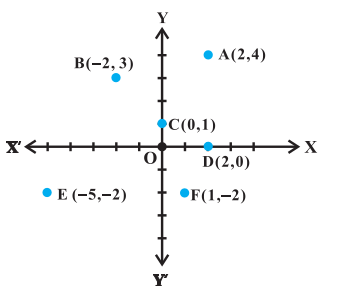
\includegraphics[scale=0.5]{1.png}

Let$ P(x,y)$ be a point in the complex plane representing the non-zero complex number $z = x +iy$ . Let $\theta$ radian
be the angle made by the directed line segment $OP$ with the positive real axis $OX$ in the anticlockwise
direction. Let $OP = r$, is known as modulus or absolute value of the complex number $z$ denoted by
$|z|$ or $mod ( z )$ .

The pair $(r,\theta)$ is known as polar coordinates of the point P.$ \theta$ is called amplitude or argument
of the complex number, denoted by $arg z$ or $amp z $.
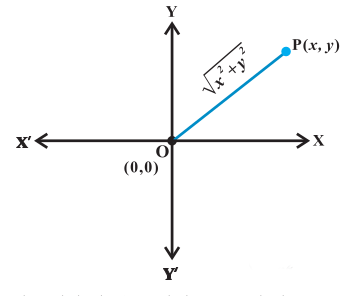
\includegraphics[scale=0.5]{2.png}

For a complex number $a+bi$ 
$$|z|=\sqrt{a^2+b^2}$$
$$tan \theta =\frac{b}{a}$$
$$\theta =tan^{-1}(\frac{b}{a})$$

\subsubsection*{Shortcut method to find arg z}
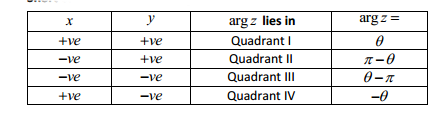
\includegraphics[scale=0.6]{3.png}
\end{multicols}
\end{document}
